\documentclass[11pt, aspectratio=169, compress]{beamer}
\usetheme[progressbar=frame title, numbering=fraction]{metropolis}      % Use metropolis theme 
\setbeamertemplate{section in toc}[sections numbered]
\setbeamertemplate{subsection in toc}[subsections numbered]
\useoutertheme[subsection=false]{miniframes}
\setbeamercolor{section in head/foot}{fg=white, bg=mDarkTeal}
\setbeamercolor{background canvas}{bg=white}
\setbeamerfont{section in head/foot}{series=\bfseries}

\usefonttheme[onlymath]{serif}
\usepackage{amsmath}
\usepackage{remreset}
\usepackage{ragged2e}
\usepackage{booktabs}
\usepackage{makecell}
\usepackage{float}
\usepackage{subfig}
\usepackage{tikz}
\usetikzlibrary{positioning,calc}
\usepackage[flushleft]{threeparttable}	% 3 part table 
\usepackage[justification=centering]{caption}
\captionsetup{skip=0pt}
\graphicspath{{./fig/}}

\makeatletter
\let\beamer@writeslidentry@miniframeson=\beamer@writeslidentry
\def\beamer@writeslidentry@miniframesoff{%
	\expandafter\beamer@ifempty\expandafter{\beamer@framestartpage}{}% does not happen normally
	{%else
		% removed \addtocontents commands
		\clearpage\beamer@notesactions%
	}
}
\newcommand*{\miniframeson}{\let\beamer@writeslidentry=\beamer@writeslidentry@miniframeson}
\newcommand*{\miniframesoff}{\let\beamer@writeslidentry=\beamer@writeslidentry@miniframesoff}
\beamer@compresstrue
\makeatother

%==============================================================
% Title Page
%==============================================================
%Information to be included in the title page:
\title{Economía social: programas y políticas de apoyo social}
\author{Rony Rodriguez-Ramírez} 
\institute{Economía Social y Humana | Grupo B018 \\Universidad Centroamericana}
\titlegraphic{\hfill
\includegraphics[height=1.5cm]{uca}}
\date{\today}
%==============================================================
\begin{document}
	
\begin{frame}[plain]
	\maketitle  
\end{frame}

%\begin{frame}{Outline}
%\tableofcontents[hideallsubsections]
%\end{frame}
%------------------------------------------------
\section{Comentarios}
%-----------------------------------------------
\subsection{Comentarios}
%-----------------------------------------------
\begin{frame}[t]{Comentarios}
Resultado del ensayo:  
\begin{itemize}
\item Media: 7.8 
\item Relación con el primer ensayo. 
\end{itemize}
Comentarios: 
\begin{itemize}
\item Etapas de los programas sociales. 
\item Contextualización de los programas sociales. Seguimiento de los beneficiarios. 
\item ¿Cuál es la mejor forma de evaluar progrmas sociales? ¿Valorización del programas? 
\item Reglas e incentivos. 
\end{itemize}
\end{frame}
%------------------------------------------------
\begin{frame}{Comentarios}
\begin{center}
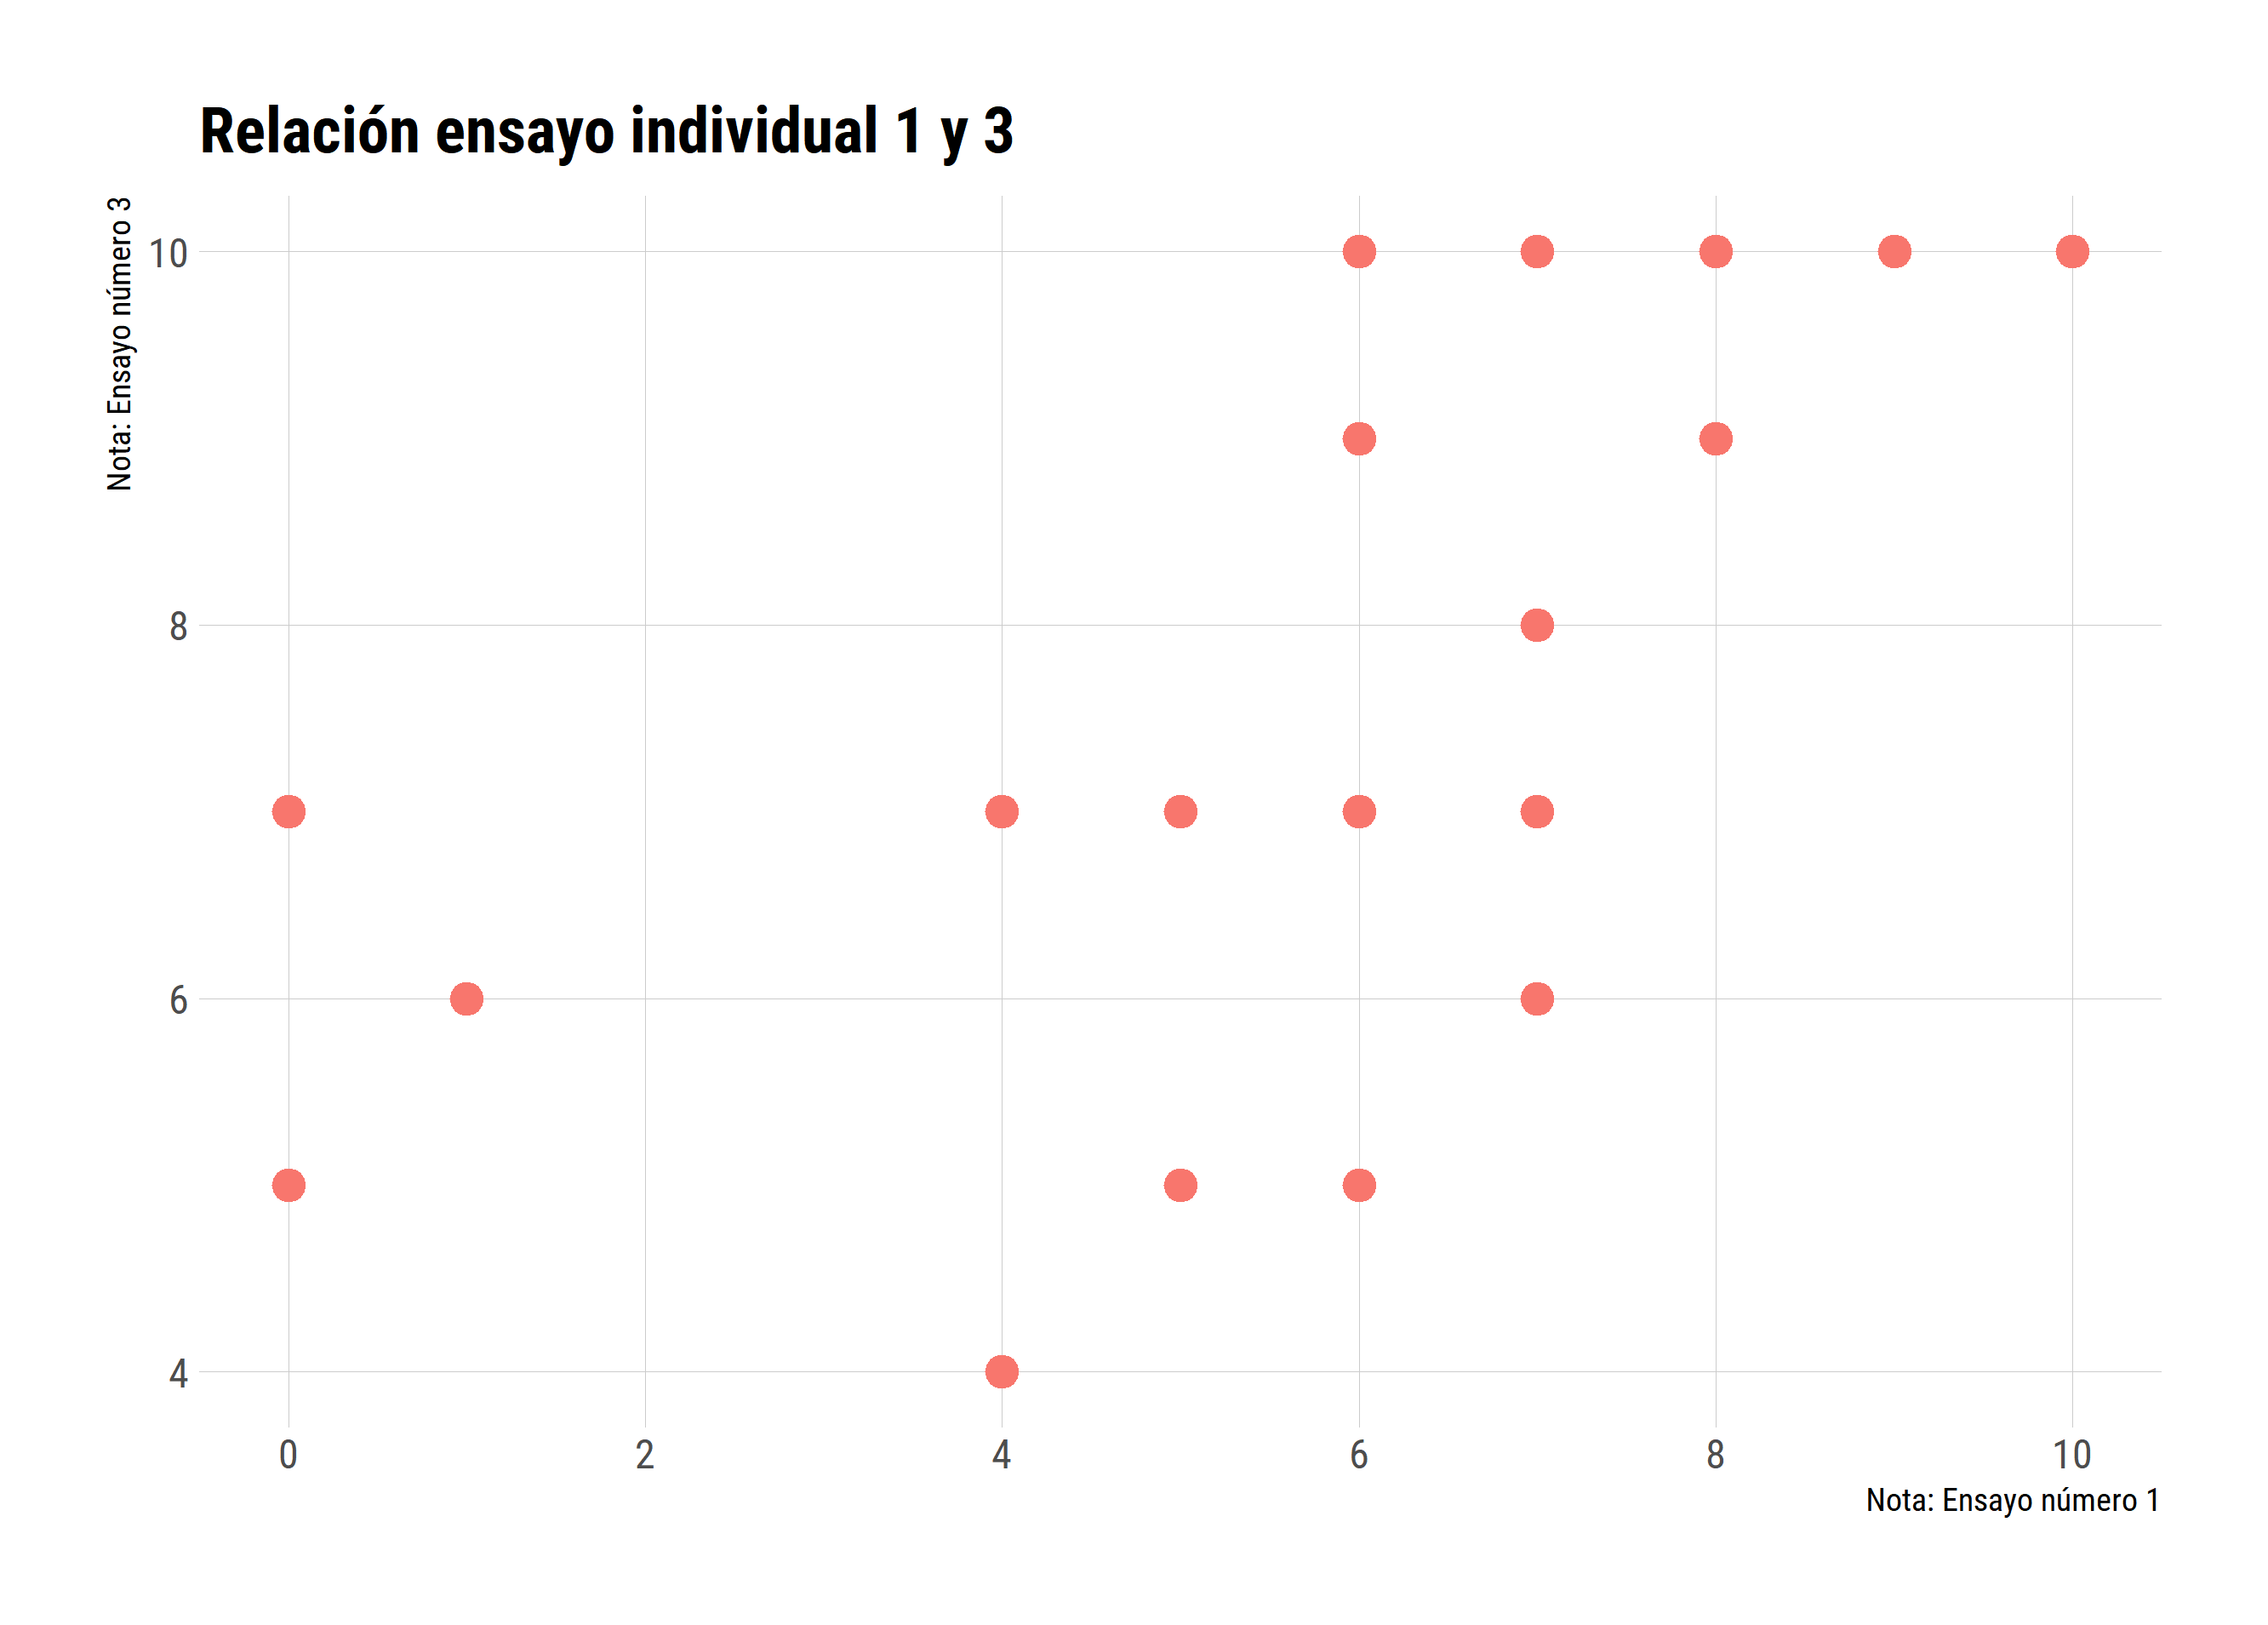
\includegraphics[width=0.7\textwidth]{fig1} 
\end{center}
\end{frame}
%------------------------------------------------
\section{Educación y racionalidad}
%------------------------------------------------
\subsection{Educación y racionalidad}
%------------------------------------------------
\begin{frame}{Racionalidad en las decisiones humanas} 
El papel de las intervenciones educativas en la mejora de la racionalidad económica: 
\begin{itemize}
	\item La racionalidad en las decisiones humanas. Supuestos y esquema tradicional. 
	\item Los humanos cometemos errores sistemáticos. 
	\item Pérdida de bienestar alta. 
	\item Repensar políticas públicas. 
\end{itemize}
\end{frame}
%------------------------------------------------
\begin{frame}{Racionalidad en las decisiones humanas} 
\textbf{Economía del comportamiento: }
\begin{itemize}
	\item Calidad de las decisiones realizadas. 
	\item La arquitectura de las decisiones. 
	\item des-sesgar nuestros conocimientos. 
\end{itemize}
¿Es esto producto de nuestro fracaso de la racionalidad o de otros factores? 

¿Qué otros factores? 
\end{frame}
%------------------------------------------------
\begin{frame}{Intervenciones educativas y racionalidad económica}
	\textbf{Efecto de la escolaridad: }
	\begin{itemize}
		\item Ingreo 
		\item Salud
		\item Crimen
	\end{itemize}
	 ¿Puede la educación mejorar nuestra toma de decisiones? 
\end{frame}
%------------------------------------------------
\begin{frame}{Intervenciones educativas y racionalidad económica}
Kim et al. (2018) examinan la siguiente hipotesis: 
\begin{itemize}
	\item Los impactos de la educación en la toma de decisiones pueden ser un mecanismo potencial subyacente a los rendimientos pecuniarios y no pecuniarios de la educación. 
\end{itemize}
Setting: 
\begin{itemize}
	\item Malawi. 
	\item Prueba controlada aleatorizada de apoyo educativo. 
	\item Solo mujeres. 
\end{itemize}
\end{frame}
%------------------------------------------------
\begin{frame}{Intervenciones educativas y racionalidad económica}
El program aleatoriamente proveía suporte financiero de educación a 2812 mujeres del 9vo y 10mo grado. 
\begin{itemize}
	\item 83 salones. 
	\item 33 escuelas públicas. 
	\item Randomizado al nivel de salón. 
\end{itemize}
El programa consistía en: 
\begin{itemize}
	\item Pago de la matrícula y tasas por 1 año. 
	\item Estipendio mensual en efectivo. 
	\item Total: \$70 por estudiante.  
\end{itemize}
\end{frame}
%------------------------------------------------
\begin{frame}{Intervenciones educativas y racionalidad económica}
\begin{itemize}
	\item Kim et al. (2018) realizaron una encuesta de seguimiento un año después para medir los efectos al corto plazo. 
	\item 4 años después realizaron una encuesta de largo plazo e implementaron experimentos de laboratorio sobre decisiones en riesgo y de tiempo.
	\item  El experimetno consistía en: 
	\begin{itemize}
		\item Riesgo: 20 problemas de decisiones representando un set de opciones de portafolio.
		\item Tiempo: cercano - 15 decisiones de alocar dinero entre mañana y 31 días; lejanos - 15 decisiones de alocar el dinero entre 1 año y 1 año y 30 días.  
	\end{itemize}
\end{itemize}
\end{frame}
%------------------------------------------------
\begin{frame}{Intervenciones educativas y racionalidad económica}
\begin{itemize}
	\item Los autores computan un indice del nivel de racional económica de los individuos. 
	\item Medido entre 0 y 1 donde 1 significa ser más consistente con la maximización de utilidad. 
\end{itemize}
\end{frame}
%------------------------------------------------
\begin{frame}{Resultados en educación}
\vspace*{-3em}
\begin{center}
	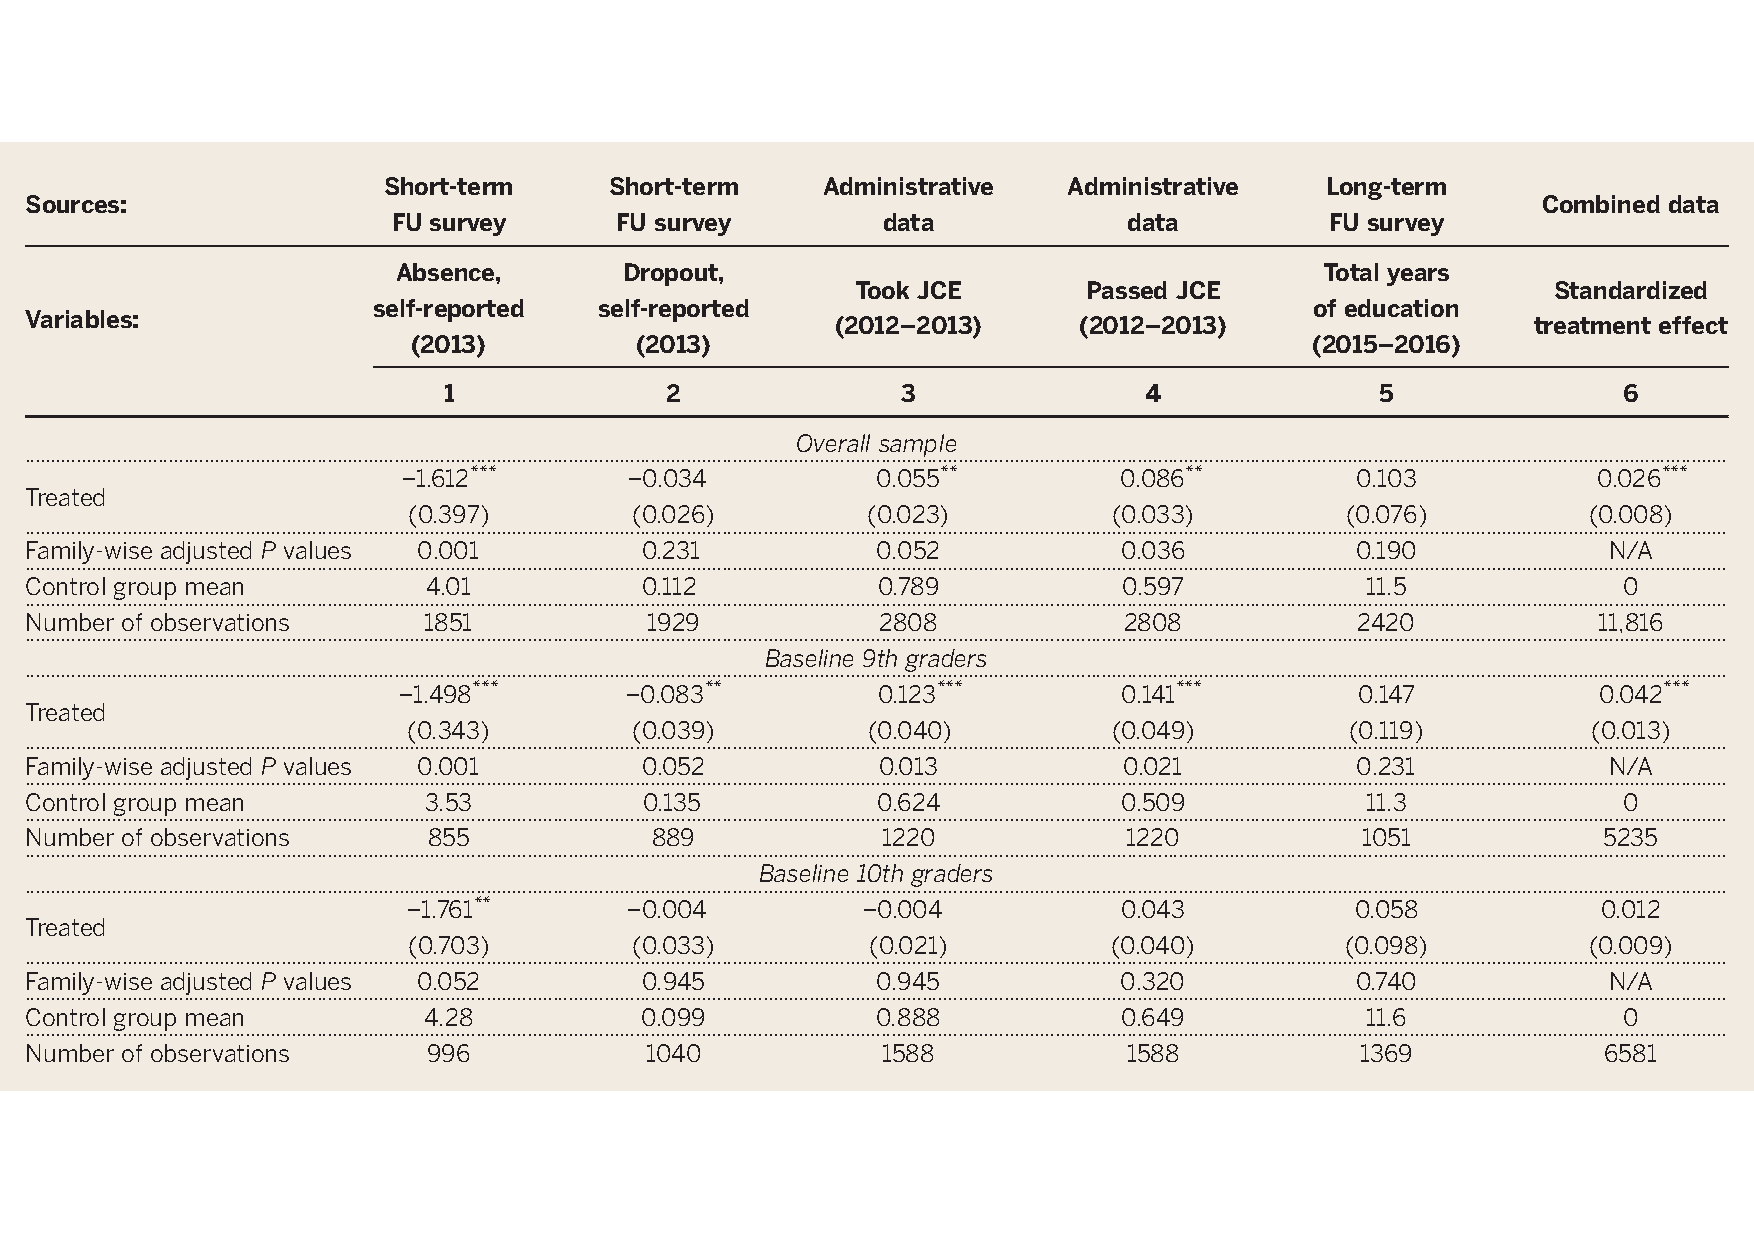
\includegraphics[width=0.9\textwidth]{tab1} 
\end{center}
\end{frame}
%------------------------------------------------
\begin{frame}{Resultados en educación}
	\begin{center}
		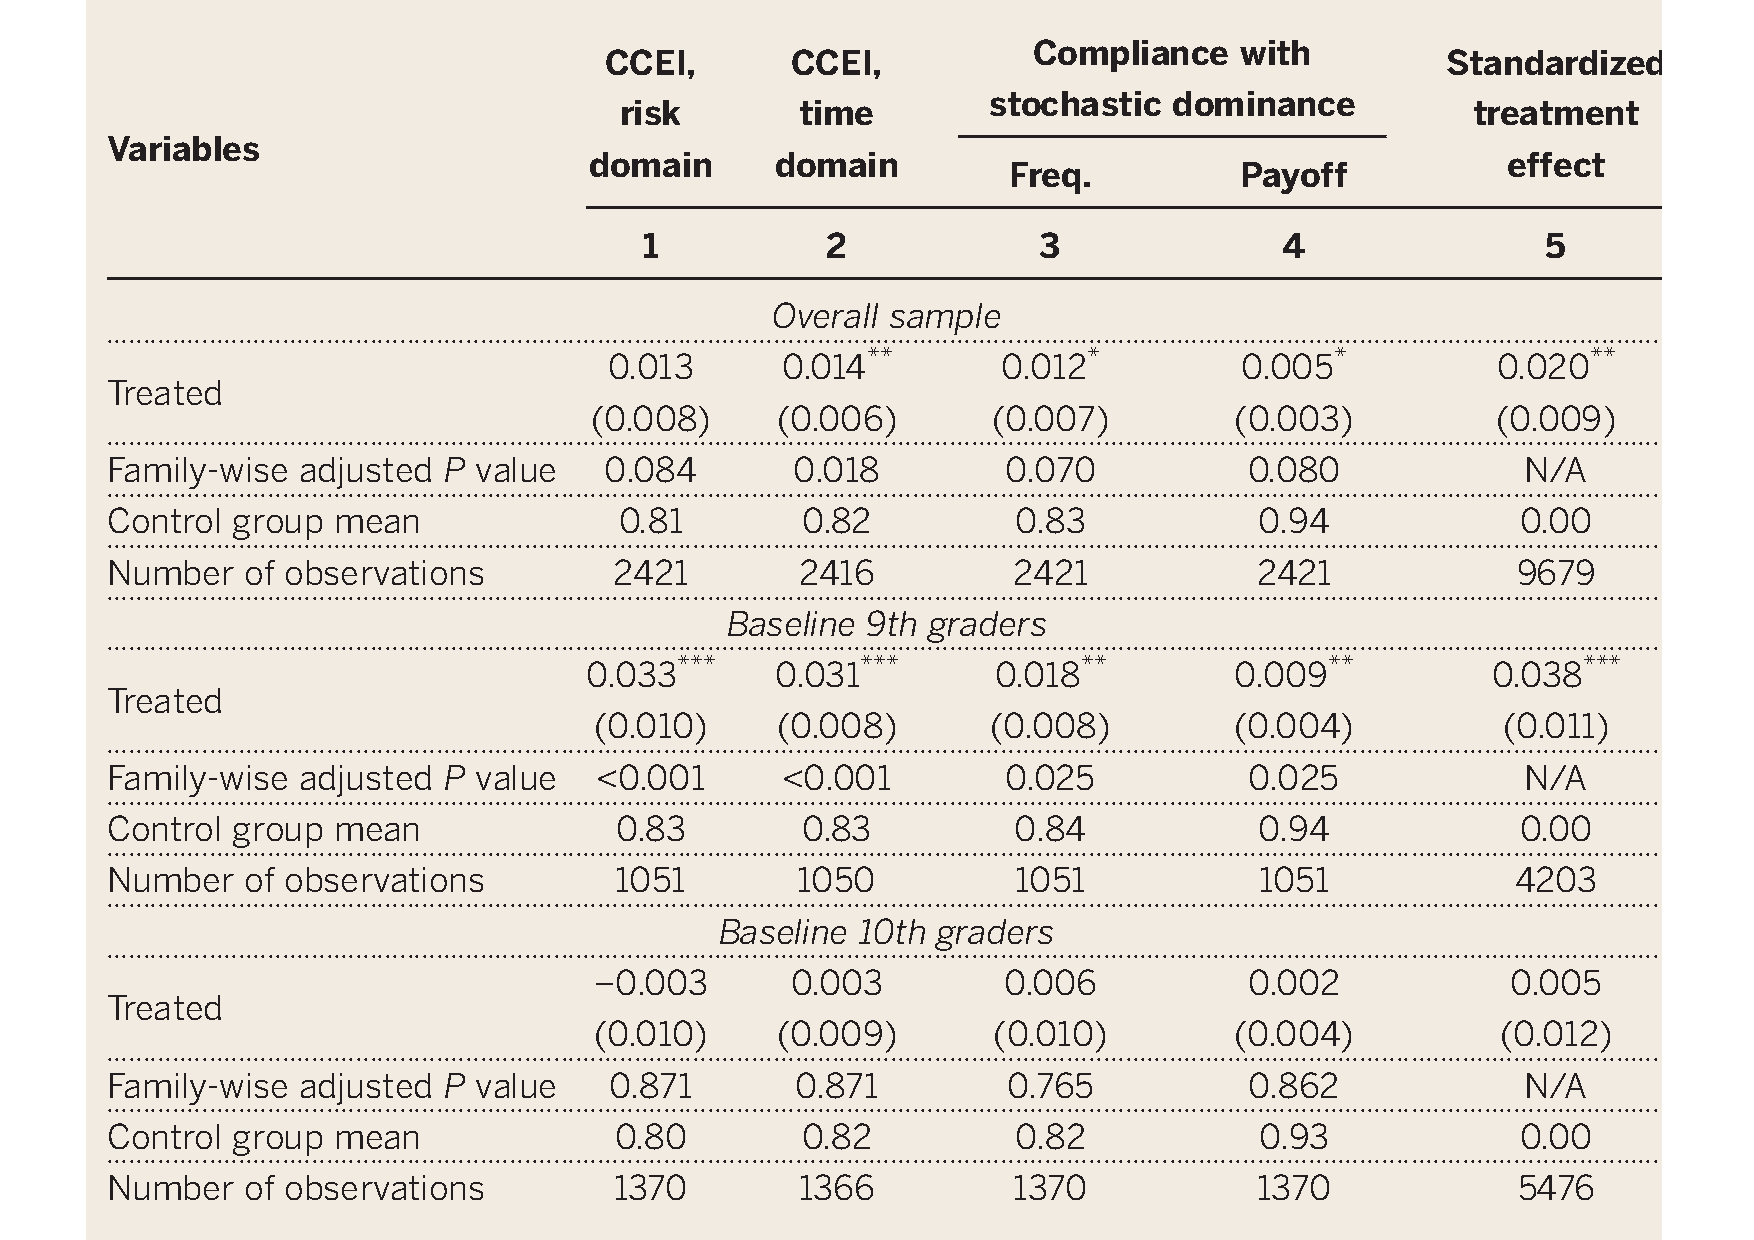
\includegraphics[width=0.7\textwidth]{tab2} 
	\end{center}
\end{frame}
%------------------------------------------------
\begin{frame}{Conclusiones}
	\begin{itemize}
		\item Evidencia causal de que una intervención educativa: 
		\begin{itemize}
			\item aumenta resultados educativos.
			\item aumenta la racionalidad económica en términos de medir la consistencia con la que las personas toman las decisiones para buscar sus objetivos económicos.
		\end{itemize}
	\item La educación puede preparar mejor a las personas para la toma de decisiones de alta calidad para sus vidas. 
	\end{itemize}
\end{frame}
%------------------------------------------------
\section{Anuncios}
\subsection{Anuncios}
%------------------------------------------------
\begin{frame}{Anuncios}
\begin{itemize}
	\item Presentacíon: 3 grupos, 22 de julio y 2 grupos el 29 (TBA). 
	\item La entrega de su presentación (pdf) debe ser el 22 de julio. 
	\item Aspectos generales de sus presentaciones. 
	\item Taller, formato. 
\end{itemize}
\end{frame}
%==============================================================
% END
%==============================================================
\miniframesoff 	
\begin{frame}[plain, standout]
Nos vemos la siguiente semana. 
\end{frame}
%------------------------------------------------
\end{document}		
